\documentclass[12pt]{scrartcl}
%\usepackage{refcheck} 
\usepackage{a4}   
\usepackage{amsmath}    
\usepackage{paralist}
\usepackage{amssymb} 
\usepackage{amsfonts}  
\usepackage{mathrsfs}  
\usepackage{dsfont}
\usepackage{latexsym} 
\usepackage{xcolor}
\usepackage{bbm,exscale}
\definecolor{Myblue}{rgb}{0,0,0.6}  
\usepackage[colorlinks,citecolor=Myblue,linkcolor=Myblue,urlcolor=Myblue,pdfpagemode=None]{hyperref}
\usepackage{amsthm}
\usepackage{accents}
\usepackage[square,numbers,sort&compress]{natbib} 
\usepackage[all,cmtip]{xy}
\usepackage{ifthen} 
\usepackage{bbding}
\usepackage{stmaryrd}  
\usepackage{wasysym}
\usepackage{verbatim}
\usepackage{bbding} 
\usepackage{soul}  %allow linebreak for underlined with \ul
\usepackage[yyyymmdd,hhmmss]{datetime}
\usepackage{tikz}
\usepackage{tikz-cd}
\usepackage{tikz-3dplot}
\usepackage{pgfplots}
	\pgfplotsset{width=7cm,compat=1.8}
	%%External
%	 \usetikzlibrary{external}\tikzexternalize
%	\usetikzlibrary{decorations.pathmorphing}
%	\usetikzlibrary{decorations.pathreplacing}
	\usetikzlibrary{decorations.markings}
%	\usetikzlibrary{calc}
%	\usetikzlibrary{fadings}
%	\usetikzlibrary{matrix} 
	\usetikzlibrary{patterns}
%	\usetikzlibrary{shapes.geometric}
%	\usetikzlibrary{shadows}

%\pgfplotsset{compat=1.11}            
            

\tikzset{
    string/.style={draw=#1, postaction={decorate}, decoration={markings,mark=at position .51 with {\arrow[color=#1]{>}}}},
    costring/.style={draw=#1, postaction={decorate}, decoration={markings,mark=at position .51 with {\arrow[draw=#1]{<}}}},
    ostring/.style={draw=#1, postaction={decorate}, decoration={markings,mark=at position .47 with {\arrow[draw=#1]{>}}}},
    ustring/.style={draw=#1, postaction={decorate}, decoration={markings,mark=at position .56 with {\arrow[draw=#1]{>}}}},
    oostring/.style={draw=#1, postaction={decorate}, decoration={markings,mark=at position .43 with {\arrow[draw=#1]{>}}}},
    uustring/.style={draw=#1, postaction={decorate}, decoration={markings,mark=at position .59 with {\arrow[draw=#1]{>}}}},
    directed/.style={string=blue!50!black}, 
    odirected/.style={ostring=blue!50!black}, 
    udirected/.style={ustring=blue!50!black}, 
    oodirected/.style={oostring=blue!50!black}, 
    uudirected/.style={uustring=blue!50!black},     
    redirected/.style={costring= blue!50!black},
    redirectedgreen/.style={costring= green!50!black},
    directedgreen/.style={string= green!50!black},
    redirectedlightgreen/.style={costring= green!65!black},
    directedlightgreen/.style={string= green!65!black},
}

\tikzset{-dot-/.style={decoration={
  markings,
  mark=at position 0.5 with {\fill circle (1.875pt);}},postaction={decorate}}}

\tikzset{
	Fdot/.style={circle, draw, fill, inner sep=0pt}, 
	Odot/.style={circle, draw, inner sep=0.1pt, minimum size=0.1cm}
	}

\def\nicedashedcolourscheme{\shadedraw[top color=blue!22, bottom color=blue!22, draw=gray, dashed]}
\def\nicedashedpalecolourscheme{\shadedraw[top color=blue!12, bottom color=blue!12, draw=gray, dashed]}
\def\nicehalfpalecolourscheme{\shadedraw[top color=blue!22, bottom color=blue!22, draw=white]}
\def\nicenotpalecolourscheme{\shadedraw[top color=blue!32, bottom color=blue!32, draw=white]}
\def\nicecolourscheme{\shadedraw[top color=blue!22, bottom color=blue!22, draw=blue!22]}
\def\nicepalecolourscheme{\shadedraw[top color=blue!12, bottom color=blue!12, draw=white]}
\def\nicenocolourscheme{\shadedraw[top color=gray!2, bottom color=gray!25, draw=white]}
\def\nicereallynocolourscheme{\shadedraw[top color=white!2, bottom color=white!25, draw=white]}
\def\boringcolourscheme{\draw[fill=blue!20, dashed]}

\newcommand\tikzzbox[1]
%{pic}% 
{#1}%#1

  \tolerance 1414
  \hbadness 1414
  \hfuzz 0.3pt
  \widowpenalty=10000
  \vfuzz \hfuzz
  \raggedbottom
  
\makeatletter
\newcommand{\raisemath}[1]{\mathpalette{\raisem@th{#1}}}
\newcommand{\raisem@th}[3]{\raisebox{#1}{$#2#3$}}
\makeatother

\renewcommand{\H}{\mathcal H}
\newcommand{\Ccal}{\mathcal C}
\newcommand{\boldB}{\boldsymbol{B}}
\newcommand{\A}{\mathcal{A}}
\newcommand{\orb}{\mathcal{A}}
\newcommand{\sgn}{\mathrm{sgn}}
\renewcommand{\leq}{\leqslant}
\renewcommand{\geq}{\geqslant}

\newcommand{\E}{\text{e}} 
\newcommand{\I}{\text{i}}
\newcommand{\B}{\mathcal{B}}
\newcommand{\Borb}{\B_{\mathrm{orb}}}
\newcommand{\Beq}{\B_{\mathrm{eq}}}
\newcommand{\C}{\mathds{C}}
\newcommand{\D}{\mathds{D}}
\newcommand{\Ee}{\mathds{E}}
\newcommand{\K}{\mathds{K}}
\newcommand{\M}{\mathds{M}}
\newcommand{\N}{\mathds{N}}
\newcommand{\Q}{\mathds{Q}}
\newcommand{\R}{\mathds{R}}
\newcommand{\Z}{\mathds{Z}}
\newcommand{\IP}{\mathds{P}}
\def\1{\ifmmode\mathrm{1\!l}\else\mbox{\(\mathrm{1\!l}\)}\fi}
\newcommand{\one}{\mathbbm{1}}
\newcommand{\be}{\begin{equation}}
\newcommand{\ee}{\end{equation}}
\newcommand{\bes}{\begin{equation*}}
\newcommand{\ees}{\end{equation*}}
\newcommand{\cc}[1] {\overline{#1}}
\newcommand{\inv}[0]{{-1}}

\newcommand{\inver}[0]{\times}%{\mathrm{inv}}
\newcommand{\chirel}[0]{\chi_{\mathrm{sym}}}%{\chi_{\frac{1}{2}}}
\newcommand{\Dec}[0]{\mathrm{Dec}}
\newcommand{\interior}[1]{%
  {\kern0pt#1}^{\mathrm{o}}%
}
\newcommand{\Strat}[0]{\mathrm{Strat}}
\newcommand{\Stratdef}[0]{\mathrm{Strat}^{\mathrm{def}}}


\newcommand{\sVir}{\mathsf{sVir}}
\newcommand{\MF}{\operatorname{MF}_{\operatorname{bi}}}
\newcommand{\MFW}{\operatorname{MF}_{\operatorname{bi}}(W)}
\newcommand{\MFR}{\operatorname{MF}^\text{R}_{\operatorname{bi}}}
\newcommand{\DG}{\operatorname{DG}_{\operatorname{bi}}}
\newcommand{\DGW}{\operatorname{DG}_{\text{bi}}(W)}
\newcommand{\DGR}{\operatorname{DG}^\text{R}_{\text{bi}}}
\newcommand{\id}{\text{id}}
\newcommand{\KMF}{K_{0}(\operatorname{MF}_{\text{bi}}}
\newcommand{\Ext}{\operatorname{Ext}}
\newcommand{\Hom}{\operatorname{Hom}}
\newcommand{\End}{\operatorname{End}}
\newcommand{\modu}{\operatorname{mod}}
\def\LG{\mathcal{LG}}
\def\LGgr{\mathcal{LG}^{\mathrm{gr}}}
\def\LGgrs{\mathcal{LG}'^{\mathrm{gr}}}
\def\LGgrso{\mathcal{LG}'^{\mathrm{gr}}_{\mathrm{orb}}}
\def\LGs{\mathcal{LG}'}
\def\LGsorb{\mathcal{LG}'_{\mathrm{orb}}}
\def\LGorb{\mathcal{LG}_{\mathrm{orb}}}
\def\LGeq{\mathcal{LG}_{\mathrm{eq}}}
\newcommand{\hmf}{\operatorname{hmf}}
\newcommand{\HMF}{\operatorname{HMF}}
\newcommand{\ev}{\operatorname{ev}}
\newcommand{\eval}{\operatorname{eval}}
\newcommand{\tev}{\widetilde{\operatorname{ev}}}
\newcommand{\coev}{\operatorname{coev}}
\newcommand{\tcoev}{\widetilde{\operatorname{coev}}}
\def\lra{\longrightarrow}
% \def\lra{%
% \;%
% %%%%%%%%%%%%%%%%%%%%%% 
% \tikzzbox{\begin{tikzpicture}[scale=1.0,color=black, >=stealth, color=black, baseline=-0.1cm]
% \draw[-{stealth[length=1.6mm, scale width=1.1]}, line width=0.15mm] (0,0) -- (0.7,0);
% \end{tikzpicture}}%%popende
% %%%%%%%%%%%%%%%%%%%%%% 
% \;%
% }
\def\lmt{\longmapsto}
\DeclareMathOperator{\tr}{tr}
\DeclareMathOperator{\str}{str}
\DeclareMathOperator{\Jac}{Jac}
\def\Re{R^{\operatorname{e}}}
\DeclareMathOperator{\Res}{Res}
\newcommand*{\longhookrightarrow}{\ensuremath{\lhook\joinrel\relbar\joinrel\rightarrow}}
\newcommand*{\twoheadlongrightarrow}{\ensuremath{\relbar\joinrel\twoheadrightarrow}}
\newcommand{\Ga}[1]{\Gamma_{\hspace{-2pt}#1}}
\newcommand{\HIA}{\Hom(I,A)}
\newcommand{\ZA}{Z_A(\Hom(I,A))}
\newcommand{\gZA}{\!Z_A^\gamma(\Hom(I,A))}
\newcommand{\gA}{{}_{\gamma_A}A}
\newcommand{\Aginv}{A_{\gamma_A^{-1}}}
\newcommand{\picc}{\pi^{(\text{c,c})}_A}
\newcommand{\pirr}{\pi^{\text{RR}}_A}
\newcommand{\tpirr}{{\widetilde\pi}^{\text{RR}}} 
\newcommand{\im}{\operatorname{im}}
\DeclareMathOperator*{\eq}{=}
\DeclareMathOperator*{\congscript}{\cong}
\newcommand{\specflow}{\mathcal U_{-\frac{1}{2},-\frac{1}{2}}}
\newcommand{\Hil}{\mathcal{H}}
\newcommand{\Hpcc}{\mathcal{H}'_{\text{(c,c)}}}
\newcommand{\Hprr}{\mathcal{H}'_{\text{RR}}}
\newcommand{\Hcc}{\mathcal{H}_{\text{(c,c)}}^A}
\newcommand{\Hrr}{\mathcal{H}_{\text{RR}}^A}
\newcommand{\HccnoA}{\mathcal{H}_{\text{(c,c)}}}
\newcommand{\HrrnoA}{\mathcal{H}_{\text{RR}}}
\newcommand{\Hrrbo}{\Hom_A(X,{}_{\gamma_A}X)}
\newcommand{\buboorb}{\beta_X^{\text{orb}}}
\newcommand{\bobuorb}{\beta^X_{\text{orb}}} 
\def\Cong{C_g}
\def\Centg{N_g}
\def\alphaKK{\alpha^{\{K\}}}
\def\alphagKg{\alpha_g^{K(g)}}
\newcommand{\AGC}{A_G^c}

\newcommand{\Bord}{\operatorname{Bord}}
\newcommand{\Bordor}{\operatorname{Bord}_{n}^{\mathrm{or}}}
\newcommand{\Borddef}{\operatorname{Bord}^{\mathrm{def}}}
\newcommand{\Borddefn}[1] {\operatorname{Bord}^{\mathrm{def}}_{#1}}
\newcommand{\Bordoc}[1] {\operatorname{Bord}^{\mathrm{oc}}_{#1}}
\newcommand{\Bords}{\operatorname{Bord}_{3}^{\APLstar}}
\newcommand{\Sphere}{\operatorname{Sphere}^{\mathrm{def}}}
\newcommand{\Nbh}{\operatorname{\mathcal{N}}}
\newcommand{\Cube}{\operatorname{Cube}}
\newcommand{\Cubed}{\operatorname{Cube}_{3}^{\mathrm{def}}(\mathds{D})}
\newcommand{\Fradj}{\operatorname{\mathcal C_{\mathds D}^{adj}}}
\newcommand{\Bordstrat}{\operatorname{Bord}^{\mathrm{strat}}}
\newcommand{\Bordstratn}[1]  {\operatorname{Bord}^{\mathrm{strat}}_{#1}}
\newcommand{\Borddlong}{\operatorname{Bord}_{3}^{\mathrm{def}}(D_3,D_2,D_1)_{s,t,f}}
\newcommand{\Bordd[1]}{\operatorname{Bord}_{#1}^{\mathrm{def}}(\mathds{D})}
\newcommand{\Strator}{\operatorname{Strat}_{n}^{\mathrm{or}}}
\newcommand{\G}{\mathcal{G}}
\newcommand{\tz}{\mathcal T_\zz}
\newcommand{\dz}{\mathcal D_\zz}
\newcommand{\tzp}{\mathcal T_{\mathcal Z'}}
\newcommand{\Data}{\mathds{D}}
\newcommand{\Obj}{\mathrm{Obj}}
\newcommand{\zz}{\mathcal{Z}}
\newcommand{\Fdp}{\operatorname{\mathcal F}_{\textrm{d}}^{\textrm{p}}}
\newcommand{\zzd}{\mathcal{Z}^{\mathrm{def}}}
\newcommand{\zztriv}{\mathcal{Z}^{\mathrm{triv}}} 
\newcommand{\zzAtriv}{\mathcal{Z}_{\mathrm{triv}}^{\Cat{A}}} 
\newcommand{\euc}{\odot}
\newcommand{\euctwo}{\odot_{\geq 2}}
\newcommand{\ieuc}{\iota^\euc}
\newcommand{\peuc}{\pi^\euc}

\newcommand{\zzTVA}{\mathcal{Z}^{TV}_{\Cat{A}}} 
\newcommand{\zzRTC}{\mathcal{Z}^{RT}_{\Cat{C}}}
\newcommand{\tzztriv}{\mathcal{T}_{{\mathcal{Z}^{triv}}}}

\newcommand{\tzGamma}{\mathcal{T}_{{\mathcal{Z}^{\Gamma}}}}
\newcommand{\unit}{\operatorname{\mathbf{1}}}  
\newcommand{\bigslant}[2]{{\raisebox{.0em}{$#1$}\left/\raisebox{-.2em}{$#2$}\right.}}
\newcommand{\Cubedp}{\operatorname{Cube}_{3}^{\mathrm{def}}(\mathds{D}')}
\newcommand{\Borddp}{\operatorname{Bord}_{3}^{\mathrm{def}}(\mathds{D}')}
\newcommand{\Vect}{\operatorname{Vect}}
\newcommand{\Vectk}{\operatorname{Vect}_\Bbbk}
\newcommand{\Alg}{\operatorname{Alg}}
\newcommand{\Algc}{\operatorname{Alg}_{\C}}
\newcommand{\Cti}{\C^\times}
\newcommand{\chiom}{\chi^\omega}
\newcommand{\CGtw}{\C^\omega[G]}

\newcommand{\eps}{\varepsilon}
\newcommand{\al}{\alpha}
\newcommand{\alb}{\overline{\alpha}}
\newcommand{\T}{\mathcal{T}}
\newcommand{\Ss}{\mathcal{S}}
\newcommand{\X}{\mathcal{X}}
\newcommand{\Y}{\mathcal{Y}}
\newcommand{\sta}{\boxempty}
\newcommand{\fus}{\otimes}
\newcommand{\sd}{^{\star}}
\newcommand{\dagg}{^{\dagger}}
\newcommand{\hash}{^{\#}}
\newcommand{\Set}{\mathrm{Set}}
\newcommand{\Ball}{\mathrm{Ball}}
\newcommand{\Sph}{\mathsf{Sph}}
\newcommand{\fork}{\pitchfork }
\newcommand{\Cat}[1]         {\operatorname{\mathcal{#1}}}
\newcommand{\Catpre}[1]         {\operatorname{\mathcal{#1}^{\mathrm{pre}}}}

\newcommand{\dX}{{}^\dagger\hspace{-1.8pt}X}
\newcommand{\dA}{{}^\dagger\hspace{-1.8pt}A}
\newcommand{\dsX}{{}^\dagger\hspace{-1.8pt}\mathcal{X}}
\newcommand{\deqX}{{}^\star\hspace{-1.8pt}X} 
\newcommand{\dseqX}{{}^\star\hspace{-1.8pt}\mathcal{X}} 
\newcommand{\dY}{{}^\dagger\hspace{-0.3pt}Y}
\newcommand{\dphi}{{}^\dagger\hspace{-0.9pt}\phi}
\newcommand{\dPhi}{{}^\dagger\hspace{-0.9pt}\Phi}

%%%%%%%%%%%%%%%%%%%%%%%%%%%%%%%%%%%%%%%%%%%%%%%%%%%%%%%%%%%%%%%%%%%%%%%%%%%%%%%% 

\newcommand{\opp}             {{\mathrm{op}}} 

%\newcommand{\Alg}        {\operatorname{\mathsf{Alg}}}
\newcommand{\Frob}        {\operatorname{\mathsf{Frob}}}
\newcommand{\Lincat}        {\operatorname{\mathsf{Cat}^{ses}}}
\newcommand{\Deftqft}{\operatorname{TQFT}^{\mathrm{def}}}

\newcommand{\KVvect}   {\operatorname{KV-2Vect}}
\newcommand{\CYvect}   {\operatorname{CY-2Vect}}

\newcommand{\evx}[1]   {\operatorname{\mathsf{ev}}_{#1}}
% coevaluation
\newcommand{\coevx}[1]   {\operatorname{\mathsf{coev}}_{#1}}
% p evaluation
\newcommand{\evp}[1]   {\operatorname{\mathsf{ev}}_{#1}^{\prime}}
% p coevaluation
\newcommand{\coevp}[1]   {\operatorname{\mathsf{coev}}_{#1}^{\prime}}

\newcommand{\evc}[1]   {\operatorname{\mathsf{c-ev}}_{#1}}
% coevaluation
\newcommand{\coevc}[1]   {\operatorname{\mathsf{c-coev}}_{#1}}
% p evaluation
\newcommand{\evpc}[1]   {\operatorname{\mathsf{c-ev}}_{#1}^{\prime}}
% p coevaluation
\newcommand{\coevpc}[1]   {\operatorname{\mathsf{c-coev}}_{#1}^{\prime}}

\def\la               {{\rm l.a.}}
\def\ra               {{\rm r.a.}}
\def\rra              {{\rm r.r.a.}}
\def\lla               {{\rm l.l.a.}}
\def\Fun              {{\mathsf{Fun}}}
\def\Funbilin              {{\mathsf{Fun}^{\mathsf{bilin}}}}

\usepackage{color}

\newcommand{\rrr}[1]{{\color{red}{#1}}}
\newcommand{\rrR}[1]{{\color{red3}{#1}}}
\newcommand{\bbb}[1]{{\color{blue}{#1}}}
\definecolor{DarkViolet} {rgb}{0.580392,0.000000,0.827450}
\newcommand{\vio}[1]{{\color{DarkViolet}{#1}}}
\newcommand{\green}[1]{{\color{green}{#1}}}



\newcommand{\ques} [1] {\marginpar\textbf{qu}\textbf{{#1} ?}} 
\newcommand{\chn}[1]{\marginpar\textbf{changed}\textbf{{#1}}}
\newcommand{\note} [1] {\marginpar\textbf{note}\textbf{{#1}}}

\newcommand{\todo} [1] {\marginpar\textbf{todo} {\bbb{#1}  } }
\newcommand{\plan} [1] {\marginpar\textbf{Plan} { \bbb{#1}  } }
%comments
\newcommand{\GS} [1] {\marginpar{\small \vio{modified\\ by GS:} {}}{ \vio{#1} }} 
\newcommand{\GSC}[1] {\marginpar{\small \vio{comment \\ by GS:} {}}{ ~\\ \it \vio{#1} \\ }} 
\newcommand{\GSQ}[1] {\marginpar{\small \vio{question\\ by GS:} {}}{ ~\\ \it \vio{#1} \\ }} 
\newcommand{\IR} [1] {\marginpar{\small \rrr{modified\\ by IR:} {}}{ \rrr{#1} }} 
\newcommand{\IRC}[1] {\marginpar{\small \rrr{comment \\ by IR:} {}}{ ~\\ \it \rrr{#1} \\ }} 
\newcommand{\IRQ}[1] {\marginpar{\small \rrr{question\\ by IR:} {}}{ ~\\ \it \rrr{#1} \\ }} 
\newcommand{\NCMod} [1] {\marginpar{\small \vio{modified\\ by NC:} {}}{ \vio{#1} }} 
\newcommand{\NCC}[1] {\marginpar{\small \vio{comment \\ by NC:} {}}{ ~\\ \it \vio{#1} \\ }} 
\newcommand{\NCQ}[1] {\marginpar{\small \vio{question\\ by NC:} {}}{ ~\\ \it \vio{#1} \\ }} 

%%%%%%%%%%%%%%%%%%%%%%%%%%%%%%%%%%%%%%%%%%%%%%%%%%%%%%%%%%%%%%%%%%%%%%%%%%%%%%%% 



\newcommand\nxt{\noindent\raisebox{.08em}{\rule{.44em}{.44em}}\hspace{.4em}}
\newcommand\arxiv[2]      {\href{http://arXiv.org/abs/#1}{#2}}
\newcommand\doi[2]        {\href{http://dx.doi.org/#1}{#2}}
\newcommand\httpurl[2]    {\href{http://#1}{#2}}

\renewcommand{\labelenumi}{(\roman{enumi})}

\allowdisplaybreaks

\deffootnote[1em]{1em}{1em}{\textsuperscript{\thefootnotemark}}

\theoremstyle{definition}
\newtheorem{definition}{Definition}
\newtheorem{proposition}[definition]{Proposition}
\newtheorem{theorem}[definition]{Theorem}
\newtheorem{theoremdefinition}[definition]{Theorem and Definition}
\newtheorem{definitionlemma}[definition]{Definition and Lemma}
\newtheorem{lemma}[definition]{Lemma}
\newtheorem{corollary}[definition]{Corollary}
\newtheorem{remark}[definition]{Remark}
\newtheorem{remarks}[definition]{Remarks}
\newtheorem{conjecture}[definition]{Conjecture}
\newtheorem{example}[definition]{Example}
\newtheorem{construction}[definition]{Construction}

\numberwithin{equation}{section}
\numberwithin{definition}{section}
\numberwithin{figure}{section}

\newcommand\void[1]{}



\begin{document}

\title{Sum${}_1$}

\author{%
\!\!\!\!\!\!\!Ilka Brunner \quad
Nils Carqueville \quad
Domenico Fiorenza \quad
}

\date{}
\maketitle

\abstract{This file contains the details on the $n=1$ case, to be merged into the main file as soon as they become polished enough.}


Let us denote by $\mathrm{Fam}_0(\mathbb{C})$ the set of equivalence classes of finite groupoids equipped with functors to $\mathbb{C}$ (seen as a trivial category). In other words, a representative of an element of $\mathrm{Fam}_0(\mathbb{C})$ is a pair $(X,\rho)$ consisting of a finite groupoid $X$ together with a map $\rho\colon \pi_0(X)\to \mathbb{C}$.
The map 
\[
\mathrm{Sum}_0\colon \mathrm{Fam}_0\to \mathbb{C}
\]
is defined as
\[
\mathrm{Sum}_0(X,\rho)=\sum_{[x]\in \pi_0(X)}\frac{\rho(x)}{|\mathrm{Aut}(x)|}.
\]
We will also use the more evocative notation
\[
\int_X \rho(x) d\mu(x)
\]
to denote $\mathrm{Sum}_0(X,\rho)$. Notice that $\mathrm{Sum}_0$ is linear in the $\rho$ variable.

%The \emph{mass} $\mu(X)$ of the finite groupoid $X$ is defined as
%\[
%\mu(X)=\mathrm{Sum}_0(X,1),
%\] 
%i.e., more explicitly,
%\[
%\mu(X)=\sum_{[x]\in \pi_0(X)}\frac{1}{|\mathrm{Aut}(x)|}.
%\]
A nice property of the morphism $\mathrm{Sum}_0$ (which we are going to use later) is the following: let $X$ be a finite set with an action of a finite group $G$, and let $X/\!/G$ denotes the action groupoid for this action; finally, let $\rho\colon X/\!/G\to \mathbb{C}$ any functor, i.e., let $\rho\colon X\to \mathbb{C}$ be a function that is constant on the $G$-orbits in $X$. Then we have
\begin{equation}\label{sum-0-on-action-groupoids}
\mathrm{Sum}_0(X/\!/G,\rho)=\frac{1}{|G|}\sum_{x\in X} \rho(x).
\end{equation}
Namely, the set $\pi_0(X/\!/G)$ is the quotient set $X/G$ and for any $x\in X$ seen as an object in $X/\!/G$ we have $\mathrm{Aut}(x)=\mathrm{Stab}_G(x)$. Therefore
\begin{align*}
\mathrm{Sum}_0(X/\!/G,\rho)&=\sum_{[x]\in X/G}\frac{\rho(x)}{|\mathrm{Stab}_G(x)|}\\
&=\frac{1}{|G|}\sum_{[x]\in X/G}\frac{|G|}{|\mathrm{Stab}_G(x)|}\rho(x)\\
&=\frac{1}{|G|}\sum_{[x]\in X/G}|[x]|\,\rho(x)\\
&=\frac{1}{|G|}\sum_{[x]\in X/G}\sum_{x\in [x]}\rho(x)\\
&=\frac{1}{|G|}\sum_{x\in X}\rho(x)
\end{align*}
\begin{remark}
A function $f\colon \pi_0(X)\to \mathbb{C}$ can equivalently be seen as an element in $\mathrm{End}_{[X,\mathrm{Vect}]}(\mathbf{1}_X)$, where $\mathbf{1}_X\colon X\to \mathrm{Vect}$ is the constant functor taking the value $\mathbb{C}$ on $X$. The map $\mathrm{Sum}_0$ can therefore be seen as the datum of a map
\[
\mathrm{Sum}_0\colon \mathrm{End}_{[X,\mathrm{Vect}]}(\mathbf{1}_X) \to \mathbb{C},
\]
for any finite groupoid $X$.
\end{remark}

\begin{definition}
The category $\mathrm{Fam}_1(\mathrm{Vect})$ has as its objects finite groupoids equipped with functors to $\mathrm{Vect}$, i.e., pairs $(X,\rho)$ consisting of a finite groupoid $X$ together with a functor $\rho\colon X\to \mathrm{Vect}$. Morphisms in $\mathrm{Fam}_1(\mathrm{Vect})$ are spans of groupoids over $\mathrm{Vect}$, i.e., commutative diagrams
\[
\xymatrix{
&Z\ar[dl]_{\pi_X}\ar[dr]^{\pi_Y}&\\
X\ar[dr]_{\rho_X}&&Y\ar[dl]^{\rho_Y}\\
&\mathrm{Vect}
\ar@{=>}_{\alpha\phantom{m}}(13,-14);(18,-14)
}
\]
where the natural transformation $\alpha\colon \rho_X\circ \pi_X\to \rho_Y\circ \pi_Y$ is part of the data of the commutative diagram.
\end{definition}
\begin{remark}
The identity mophisms and the composition of morphisms in $\mathrm{Fam}_1(\mathrm{Vect})$ will be defined later.
\end{remark}

For every object $(X,\rho)$ in $\mathrm{Fam}_1(\mathrm{Vect})$ we can consider the vector space 
\[
[\mathbf{1}_X,\rho]=\mathrm{Hom}_{[X,\mathrm{Vect}]}(\mathbf{1}_X,\rho).
\]
If $f\colon Y\to X$ is a functor between finite groupoids, and $\rho\colon X\to \mathrm{Vect}$ is a functor, we write $f^*\rho\colon Y\to \mathrm{Vect}$ for the functor $\rho\circ f$. If $\alpha\colon \mathbf{1}_X\to \rho$ is a natural transformation, then $f^*\alpha$ is a natural transformation between $f^*\mathbf{1}_X=\mathbf{1}_Y$ and $f^*\rho$. This defines a linear map
\[
f^* \colon [\mathbf{1}_X,\rho] \to [\mathbf{1}_Y, f^*\rho].
\]
Similarly, we can consider the vector space
\[
[\rho,\mathbf{1}_X]=\mathrm{Hom}_{[X,\mathrm{Vect}]}(\rho, \mathbf{1}_X)
\]
together with the linear map 
\[
f^* \colon [\rho,\mathbf{1}_X] \to [f^*\rho,\mathbf{1}_Y].
\]
Passing to the linear duals we get the linear map
\[
(f^*)^\vee\colon [f^*\rho,\mathbf{1}_Y]^\vee \to [\rho,\mathbf{1}_X]^\vee.
\]
Next, notice that composition of morphisms gives a bilinear map
\[
[\rho,\mathbf{1}_X]\otimes [\mathbf{1}_X,\rho] \to [\mathbf{1}_X,\mathbf{1}_X]
\]
and so composing this with the linear map $\mathrm{Sum}_0(X,-)\colon [\mathbf{1}_X,\mathbf{1}_X]\to \mathbb{C}$ we get a bilinear pairing $\langle\,|\,\rangle_X$ between $[\rho,\mathbf{1}_X]$ and $[\mathbf{1}_X,\rho]$, for any $\rho$. Notice that, by its very definition, the pairing $\langle\,|\,\rangle_X$ satisfies
\[
\langle v|\alpha\circ w\rangle_X =\langle  v\circ \alpha|w \rangle_X,
\]
for any $v\in [\rho_2,\mathbf{1}_X]$, any $w\in [\mathbf{1}_X,\rho_1]$ and any natural transformation $\alpha\colon \rho_1\to \rho_2$.
Equivalently, the bilinear pairing $\langle\,|\,\rangle_X$ is a linear map
\[
\delta_{(X,\rho)}\colon [\mathbf{1}_X,\rho]\to [\rho,\mathbf{1}_X]^\vee.
\]
Our main \emph{duality assumption} will be that $\delta_{(X,\rho)}$ is a linear isomorphism for any $(X,\rho)$. 
\begin{remark}
The duality assumption holds for every finite groupoid $X$ if and only if it holds for finite connected groupoids. Up to equivalence we are therefore reduced to considering the case $X=\mathbf{B}G$, with $G$ a finite group. In this case $\rho\colon \mathbf{B}G\to \mathrm{Vect}$ is the datum of a linear representation $V$ of $G$, and the vector spaces $[\mathbf{1}_{\mathbf{B}G},\rho]$ and $[\rho,\mathbf{1}_{\mathbf{B}G}]$ are isomorphic to the space $V^G$ of $G$-invariants and the linear dual $(V_G)^\vee$ of the space of $G$-coinvariants, respectively. The map $\delta_{(\mathbf{B}G,\rho)}$ is therefore a map
\[
\delta_{(\mathbf{B}G,\rho)}\colon V^G\to (V_G)^{\vee\vee}\cong V_G,
\]
from $G$-invariants to $G$-coinvariants. Let $v\mapsto [v]$ be the canonical projection $V\to V_G=V/\langle v-g\cdot v\rangle_{v\in V;g\in G}$. By composing with the inclusion $V^G\hookrightarrow V$ we get the morphism $\iota\colon v\mapsto [v]$ from $V^G\to V_G$. This is an isomorphism. Indeed, the canonical projection $\pi\colon V\to V^G$ given by
\[
\pi\colon v\mapsto \frac{1}{|G|}\sum_{g\in G} g\cdot v
\]
is zero on the elements of the form $v-g\cdot v$ and so induces a linear map $\tilde{\pi}\colon V_G\to V^G$, which is immediate to see is the inverse of $\iota$.
For any $w\in (V_G)^\vee$ seen as an element in $[\rho,\mathbf{1}_{\mathbf{B}G}]$ and any $v\in V^G$ seen as an element in $[\mathbf{1}_{\mathbf{B}G},\rho]$ we have $w\circ v =w([v])$ Therefore
\[
\langle w| v\rangle_{\mathbf{B}G}=\frac{1}{|G|}w\circ v=w\left(\frac{1}{|G|}\iota(v)\right).
\]
This means that $\delta_{(\mathbf{B}G,\rho)}v$ is the evaluation on $\frac{1}{|G|}\iota(v)$. Therefore, under the canonical isomorphism $(V_G)^{\vee\vee}\cong V_G$, we have $\delta_{(\mathbf{B}G,\rho)}=\frac{1}{|G|}\iota$. As $\iota$ is an isomorphism, so is $\delta_{(\mathbf{B}G,\rho)}$.
\end{remark}

Under the duality assumption we may define a linear morphism 
\[
f_*\colon [\mathbf{1}_Y,f^*\rho]\to  [\mathbf{1}_X,\rho]
\]
as the composition
\[
[\mathbf{1}_Y,f^*\rho]\xrightarrow{\delta_{(Y,f^*\rho)}}[f^*\rho,\mathbf{1}_Y]^\vee \xrightarrow{(f^*)^\vee} [\rho,\mathbf{1}_X]^\vee \xrightarrow{\delta_{(X,\rho)}^{-1}} [\mathbf{1}_X,\rho].
\]
In other words, if $v\in [\mathbf{1}_Y,f^*\rho]$, the element $f_*v\in [\mathbf{1}_X,\rho]$ is defined 
%by the equation
%\[
%\int_X (w\circ f_*(v)) d\mu(x) = \int_Y((f^*w)\circ v) d\mu(y),
%\]
%i.e.,
 by the equation
\[
\langle w| f_*v\rangle_X = \langle f^*w| v\rangle_Y
\]
for any $w\in [\rho,\mathbf{1}_X]$. Similarly, we have a morphism $f_*\colon [f^*\rho,\mathbf{1}_Y]\to [\rho,\mathbf{1}_X]$ defined by
\[
\langle f_*w| v\rangle_X = \langle w| f^*v\rangle_Y.
\]


We can now define our wannabe functor
\[
\mathrm{Sum}_1\colon \mathrm{Fam}_1(\mathrm{Vect})\to \mathrm{Vect}
\]
on objects as 
\[
\mathrm{Sum}_1(X,\rho)=[\mathbf{1}_X,\rho]
\]
and on a morphism 
\[
\xymatrix{
&Z\ar[dl]_{\pi_X}\ar[dr]^{\pi_Y}&\\
X\ar[dr]_{\rho_X}&&Y\ar[dl]^{\rho_Y}\\
&\mathrm{Vect}
\ar@{=>}_{\alpha\phantom{m}}(13,-14);(18,-14)
}
\]
as the composition
\[
[\mathbf{1}_X,\rho_X]\xrightarrow{\pi_X^*} [\mathbf{1}_Z,\pi_X^*\rho_X]\xrightarrow{\alpha\circ-}  [\mathbf{1}_Z,\pi_Y^*\rho_Y] \xrightarrow{\pi_{Y*}} [\mathbf{1}_Y,\rho_Y].
\]

\begin{remark}
Before giving a more explicit expression of the above morphism, let us notice that $[\mathbf{1}_X,\rho]$ is a model for the limit of the functor $\rho\colon X\to \mathrm{Vect}$, in accordance with the prescrition in \cite{FHLT}. Also, notice that the morphism associated to the span $X\leftarrow Z\to Y$ together with the natural transformation $\alpha$ has the form ``pull-compose-push'', and so it is an instance of a Fourier-Mukai-type transform.
\end{remark}



\begin{lemma} (The projection formula)
\label{lem:projectionformula}
Let $f\colon Y\to X$ be a functor between finite groupoids, let $\rho_1,\rho_2\colon X\to \mathrm{Vect}$ be functors and let $\alpha\colon \rho_1\to\rho_2$ be a natural transformation. We have an identity of morphisms $[\mathbf{1}_Y,f^*\rho_1]\to [\mathbf{1}_X,\rho_2]$
\[
f_*(f^*\alpha\circ -) = \alpha\circ f_*
\] 
\end{lemma}
\begin{proof}
The identity
\[
f_*(f^*\alpha\circ v) = \alpha\circ f_*v
\]
for every $v\in [\mathbf{1}_Y,f^*\rho_1]$ is equivalent to the identity
\[
\langle w| f_*(f^*\alpha\circ v)\rangle_X = \langle w|\alpha\circ f_*v\rangle_X
\]
for every $v\in [\mathbf{1}_Y,f^*\rho_1]$ and every $w\in [\rho_2,\mathbf{1}_X]$. By the properties of the pairings $\langle\,|\,\rangle_X$ and $\langle\,|\,\rangle_X$, and by definition of $f_*$, we have
\begin{align*}
\langle w| f_*(f^*\alpha\circ v)\rangle_X&=\langle f^*w| f^*\alpha\circ v\rangle_Y\\
&=\langle f^*w\circ f^*\alpha| v\rangle_Y\\
&=\langle f^*(w\circ \alpha)| v\rangle_Y\\
&=\langle w\circ \alpha| f_*v\rangle_X\\
&=\langle w| \alpha \circ f_*v\rangle_X
\end{align*}
\end{proof}

For  later use, let us derive an explicit formla for $f_*$ in case $f\colon \mathbf{B}G\to \mathbf{B}H$ is a morphism of finite groups (seen as groupoids with a single object).

 Recall that  if $v\in [\mathbf{1}_Y,f^*\rho]$, the element $f_*v\in [\mathbf{1}_X,\rho]$ is defined 
 by the equation $
\langle w| f_*v\rangle_{\mathbf{B}H} = \langle f^*w| v\rangle_{\mathbf{B}G}$
for any $w\in [\rho,\mathbf{1}_X]$. As both $\mathbf{B}G$ and $\mathbf{B}H$ have a single object, this equation reduces to
\[
\frac{w\circ f_*v}{|H|}=\frac{f^*w\circ v}{|G|}
\] 
The morphism $\rho\colon \mathbf{B}H\to \mathrm{Vect}$ is the datum of a linear representation of $H$ on a vector space $V$, and $f^*\rho$ is the datum of representation of $G$ obtained by pull-back, i.e., the group $G$ acts on $V$ by $g\cdot \xi := f(g)\cdot \xi$. The element $v\in [\mathbf{1}_Y,f^*\rho]$ is therefore a $G$-invariant vector of $V$, while $w\in [\rho,\mathbf{1}_X]$ is a linear functional on $V$ factoring through the space of $H$-coinvariants. The element $f^*w$ is the same linear functional on $V$, but this time seen as factoring through the space of $H$-coinvariants. Therefore the composition $f^*w\circ v$ is just the evaluation of $w\colon V\to \mathbb{C}$ on the vector $v\in V$, under the canonical isomorphism $\mathrm{End}(\mathbb{C})\cong \mathbb{C}$. Finally, $f_*v\in  [\mathbf{1}_X,\rho]$ is an $H$-invariant vector of $V$, and $w\circ f_*v$ is the evaluation of $w\colon V\to \mathbb{C}$ on the vector $f_*v\in V$. The defining equation for $f_*v$ then becomes
\[
w\left(\frac{f_*v}{|H|}\right)=w\left(\frac{v}{|G|}\right)
\] 
for any $w\colon V\to \mathbb{C}$ factoring through the space of $H$-coinvariants.
From $v/|G|$ we get the $H$-invariant vector 
\[
\frac{1}{|H|}\sum_{h\in H}h\cdot \frac{v}{|G|}
\]
and, since $w$ factors through the $H$-coinvariants,
\[
w\left(\frac{v}{|G|}\right)=w\left(\frac{1}{|H|}\sum_{h\in H}h\cdot \frac{v}{|G|}\right)
\]
The defining equation for $f_*v$ can therefore be rewritten as
\[
\langle w| f_*v\rangle_{\mathbf{B}H}=\langle w| \sum_{h\in H}\frac{h\cdot v}{|G|}\rangle_{\mathbf{B}H},
\]
for any $w\in [\rho,\mathbf{1}_X]$. As the pairing $\langle \,| \,\rangle_{\mathbf{B}H}$ is nondegenerate, this finally gives
\[
f_*v=\frac{1}{|G|}\sum_{h\in H} h\cdot v.
\] 

\begin{remark}
This formula simplifies a bit in case the group homomorphism $f\colon G\to H$ is surjective. Indeed, in that case, the $G$-invariant vector $v$ will be automatically $H$-invariant and we find
\[
f_*v=\frac{|H|}{|G|} v
\]
in this case.
\end{remark}

\begin{lemma}
\label{lem:BeckChevalley}
Consider a homotopy pullback diagram of finite groupoids
\[
\xymatrix{
& X\times_TY\ar[dl]_{p_1}\ar[dr]^{p_2}\\
X\ar[dr]_{f_1}&& Y\ar[dl]^{f_2}
\\& T
\ar@{=>}_{\eta\phantom{m}}(13,-14);(18,-14)
}
\]
and a morphism $\rho\colon T\to \mathrm{Vect}$.
Then the Beck-Chevalley condition is satisfied, i.e., we have an identity of morphisms $f_2^*f_{1*}=p_{2*}(\eta^*\rho\circ-)p_1^*$ from $[\mathbf{1}_X,f_1^*\rho]$ to $[\mathbf{1}_Y,f_2^*\rho]$.
\end{lemma}

\begin{proof}
By restricting to connected components, and working up to equivalence of finite groupoids, we may assume that the given pullback diagram has the form
\[
\xymatrix{
& G\backslash\!\backslash H/\!/K\ar[dl]_{p_1}\ar[dr]^{p_2}\\
\mathbf{B}G\ar[dr]_{f_1}&& \mathbf{B}K\ar[dl]^{f_2}
\\& \mathbf{B}H
\ar@{=>}_{\eta\phantom{m}}(13,-14);(18,-14)
}
\]
where the natural transformation $\eta$ is defined by $\eta_h=h$; this precisely expresses the fact that a morphism from $h$ to $h'$ in the action groupoid  $G\backslash\!\backslash H/\!/K$ is given by a commutative diagram
\[
\xymatrix{
\ast\ar[r]^{h}\ar[d]_{f_1(g)}&\ast\ar[d]^{f_2(k)}\\
\ast\ar[r]_{h'}&\ast
}.
\]
The equation $f_2^*f_{1*}=p_{2*}(\eta^*\rho\circ-)p_1^*$ is equivalent to $\langle w| f_2^*f_{1*}v\rangle_{\mathbf{B}K} = \langle w|p_{2*}(\eta^*\rho\circ p_1^*v)\rangle_{\mathbf{B}K}$ for any $v\in [\mathbf{1}_{\mathbf{B}G},f_1^*\rho]$ and any $w\in [f_2^*\rho,\mathbf{1}_{\mathbf{B}K}]$. This is equivalent to the equation
\[
\langle f_{2*}w| f_{1*}v\rangle_{\mathbf{B}H} = \langle p_2^*w|\eta^*\rho\circ p_1^*v\rangle_{G\backslash\!\backslash H/\!/K}.
\]
The morphism $\rho\colon \mathbf{B}H\to \mathrm{Vect}$ is the datum of a linear representation of the finite group $H$ on a vector space $V$. The element $v$ is a $G$-invariant vector of $V$ (where $G$ acts on $V$ via $f_1$) and $w$ is a linear functional on $V$ which factors through the $K$-coinvariants (with $K$ acting via $f_2$). By the above explicit formula for $f_*$ in the case of a group morphism, we have
\[
f_{1*}v=\frac{1}{|G|}\sum_{h\in H} h\cdot v;\qquad f_{2*}w=\frac{1}{|K|}\sum_{h\in H} h\cdot w,
\]
where on the right we have the $H$-action on linear functionals on $V$, i.e., $(h\cdot w)= w(h^{-1}\cdot -)$. We therefore find
\begin{align*}
\langle f_{2*}w| f_{1*}v\rangle_{\mathbf{B}H}&=\frac{1}{|H||G||K|}\sum_{h_1,h_2\in H}w(h_1^{-1}h_2\cdot v)\\
&=\frac{1}{|H||G||K|}\sum_{h\in H}\sum_{h_1^{-1}h_2=h}w(h_1^{-1}h_2\cdot v)\\
&=\frac{1}{|H||G||K|}\sum_{h\in H}\sum_{h_1\in H}w(h\cdot v)\\
&=\frac{1}{|G||K|}\sum_{h\in H}w(h\cdot v)
\end{align*}

To every object $h$ of $G\backslash\!\backslash H/\!/K$, the functors $p_1^*f_1^*\rho$ and $p_2^*f_2^*\rho$ both assign the vector space $V$, so $p_1^*v$ and $p_2^*w$ consist in a copy of the vector $v$ and of the linear functional $w\colon V\to \mathbb{C}$ for each of the copies of $V$ associated with the elements of $H$. Moreover, since $\eta_h=h$, the natural transformation $\eta^*\rho=\rho\circ\eta$ at the object $h$ is precisely the multiplication by $h$ as a linear map from $V$ to $V$. This means that $\eta^*\rho\circ p_1^*v=(h\cdot v)_{h\in H}$, i.e, $\eta^*\rho\circ p_1^*v$  consists of the choice of the vector $h\cdot v$ in the copy of $V$ associated with the object $h$ of $G\backslash\!\backslash H/\!/K$. We therefore find
\begin{align*}
\langle p_2^*w|\eta^*\rho\circ p_1^*v\rangle_{G\backslash\!\backslash H/\!/K}=\frac{1}{|G||K|}\sum_{h\in H}w(h\cdot v),
\end{align*}
by the formula \eqref{sum-0-on-action-groupoids}.
\end{proof}

%Let us now give an explicit description of the functor $\mathrm{Sum}_1$. To begin with, notice that the datum of a functor $\rho\colon X\to \mathrm{Vect}$ is equivalent to the datum of a linear representation $V_x$ of $\mathrm{Aut}_X(x)$ for every $x$ in a set of representatives for the isomophism classes of objects in $X$. So 
%\[
%[\mathbf{1}_X,\rho]=\bigoplus_{[x]\in \pi_0(X)}(V_x)^{\mathrm{Aut}_X(x)},
%\]
%where $V^G$ denotes the subspace of $G$-invariants for a linear $G$-representation on a vector space $V$. A linear map $[\mathbf{1}_X,\rho_X]\to [\mathbf{1}_Y,\rho_Y]$ can therefore be described by its ``matrix coefficients'' $ (V_x)^{\mathrm{Aut}_X(x)}\to (W_y)^{\mathrm{Aut}_Y(y)}$ with $[x]$ ranging in $\pi_0(X)$ and $[y]$ ranging in $\pi_0(Y)$. The map
%$\pi_X^*\colon [\mathbf{1}_X,\rho_X]\to [\mathbf{1}_Z,\pi_X^*\rho_X]$ maps the invariant vector $v_x$ in $V_x$ to the tuple $(v_x,v_x,\dots,v_x)$ in $\bigoplus_{\pi_X([z])=[x]}V_x$. In this vector space, look at the direct sum over those $[z]$ with $\pi_Y([z])=[y]$. These are precisely those summands for which $\alpha_z$ is a linear morphism $V_x\to W_y$. The corresponding tuple $(\alpha_{z_1}(v_x),\alpha_{z_2}(v_x),\dots, \alpha_{z_k}(v_x))$ is then the component of $(\alpha\circ\pi_X^*)(v_x)$ in $[\mathbf{1}_Z,\pi_Y^*\rho_Y]$ going into $W_y$ via $\pi_{Y*}$. As shown above, the mophism $\pi_{Y*}$ acts on this component by mapping it to
%\[
%\sum_{\substack{\pi_X([z])=[x]\\ \pi_Y([z])=[y]}} \sum_{h\in \mathrm{Aut}(y)}\frac{h\cdot \alpha_z(v_x)}{|\mathrm{Aut}(z)|} . 
%\]
%In other words, the matrix coefficient
%\[
%(\Phi_\alpha)_x^y\colon (V_x)^{\mathrm{Aut}_X(x)}\to (W_y)^{\mathrm{Aut}_Y(y)}
%\]
%is
%\[
%v_x\mapsto 
%\sum_{\substack{\pi_X([z])=[x]\\ \pi_Y([z])=[y]}} \sum_{h\in \mathrm{Aut}(y)}\frac{h\cdot \alpha_z(v_x)}{|\mathrm{Aut}(z)|} .
%\]
%Notice that on the right hand side we have an integral over the groupoid $Z_{x,y}$ given by the (homotopy) fiber of $Z$ over the point $(x,y)$ of $X\times Y$. This exhibits the ``propagator'' $(\Phi_\alpha)_{xy}$ as the ``sum of $\alpha$ over the histories $z$ going from $x$ to $y$'' (averaged over $\mathrm{Aut}(y)$), and so as a discrete version of the Feynman path integral expression for propagators in quantum field theory.
%

\begin{proposition}
$\textrm{Sum}_1$ is a functor $\textrm{Fam}_1(\Vect) \to \Vect$. 
\end{proposition}

\begin{proof}
We have the verify that $\textrm{Sum}_1$ is compatible with units and composition. 
Let $\alpha \colon \rho_1 \to \rho_2$ and $\beta \colon \rho_2 \to \rho_3$ be composable morphisms in $\textrm{Fam}_1(\Vect)$: 
$$
%%%%%%%%%%%%%%%%%%%%%%%
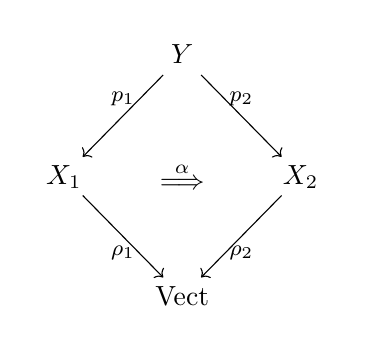
\begin{tikzpicture}[
			     baseline=(current bounding box.base), 
			     %>=stealth,
			     descr/.style={fill=white,inner sep=3.5pt}, 
			     normal line/.style={->}
			     ] 
\matrix (m) [matrix of math nodes, row sep=3.0em, column sep=2em, text height=1.5ex, text depth=0.1ex] {%
{} & Y & {} 
\\
X_1 & {} & X_2 
\\
{} & \Vect & {} 
\\
};
\path[font=\footnotesize] (m-1-2) edge[->] node[above] {$p_1$} (m-2-1);
\path[font=\footnotesize] (m-1-2) edge[->] node[above] {$p_2$} (m-2-3);
\path[font=\footnotesize] (m-2-1) edge[->] node[below] {$\rho_1$} (m-3-2);
\path[font=\footnotesize] (m-2-3) edge[->] node[below] {$\rho_2$} (m-3-2);
\fill (0,0) circle (0pt) node {$\stackrel{\alpha}{\implies}$};
\end{tikzpicture}
%%%%%%%%%%%%%%%%%%%%%%% 
\! , \quad 
%%%%%%%%%%%%%%%%%%%%%%%
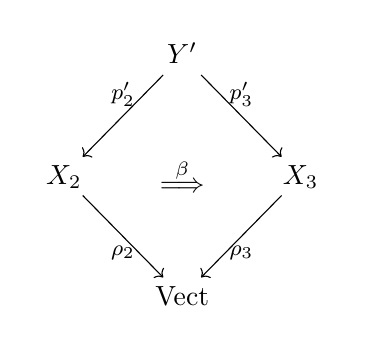
\begin{tikzpicture}[
			     baseline=(current bounding box.base), 
			     %>=stealth,
			     descr/.style={fill=white,inner sep=3.5pt}, 
			     normal line/.style={->}
			     ] 
\matrix (m) [matrix of math nodes, row sep=3.0em, column sep=2em, text height=1.5ex, text depth=0.1ex] {%
{} & Y' & {} 
\\
X_2 & {} & X_3 
\\
{} & \Vect & {} 
\\
};
\path[font=\footnotesize] (m-1-2) edge[->] node[above] {$p'_2$} (m-2-1);
\path[font=\footnotesize] (m-1-2) edge[->] node[above] {$p'_3$} (m-2-3);
\path[font=\footnotesize] (m-2-1) edge[->] node[below] {$\rho_2$} (m-3-2);
\path[font=\footnotesize] (m-2-3) edge[->] node[below] {$\rho_3$} (m-3-2);
\fill (0,0) circle (0pt) node {$\stackrel{\beta}{\implies}$};
\end{tikzpicture}
%%%%%%%%%%%%%%%%%%%%%%% 
\! .
$$%
Then by definition of $\textrm{Fam}_1(\Vect)$, their composition $\beta \circ_\eta \alpha$ is the natural transformation $(\beta * 1_{\pi_2}) \cdot (1_{\rho_2} * \eta) \cdot (\alpha * 1_{\pi_1})$: 
$$
\beta \circ_\eta \alpha 
\; \stackrel{\text{def}}{=} \; 
%%%%%%%%%%%%%%%%%%%%%%%
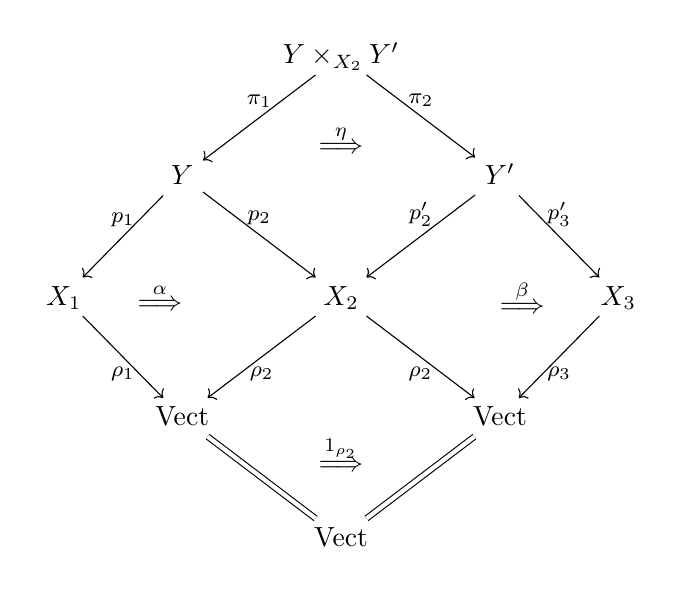
\begin{tikzpicture}[
			     baseline=(current bounding box.base), 
			     %>=stealth,
			     descr/.style={fill=white,inner sep=3.5pt}, 
			     normal line/.style={->}
			     ] 
\matrix (m) [matrix of math nodes, row sep=3.0em, column sep=2em, text height=1.5ex, text depth=0.1ex] {%
{} & {} & Y \times_{X_2} Y' & {} & {}
\\
{} & Y & {} & Y' & {}
\\
X_1 & {} & X_2 & {} & X_3
\\
{} & \Vect & {} & \Vect & {}
\\
{} & {} & \Vect & {} & {}
\\
};
\path[font=\footnotesize] (m-1-3) edge[->] node[above] {$\pi_1$} (m-2-2);
\path[font=\footnotesize] (m-1-3) edge[->] node[above] {$\pi_2$} (m-2-4);
\path[font=\footnotesize] (m-2-2) edge[->] node[above] {$p_1$} (m-3-1);
\path[font=\footnotesize] (m-2-2) edge[->] node[above] {$p_2$} (m-3-3);
\path[font=\footnotesize] (m-2-4) edge[->] node[above] {$p'_2$} (m-3-3);
\path[font=\footnotesize] (m-2-4) edge[->] node[above] {$p'_3$} (m-3-5);
\path[font=\footnotesize] (m-3-1) edge[->] node[below] {$\rho_1$} (m-4-2);
\path[font=\footnotesize] (m-3-3) edge[->] node[below] {$\rho_2$} (m-4-2);
\path[font=\footnotesize] (m-3-3) edge[->] node[below] {$\rho_2$} (m-4-4);
\path[font=\footnotesize] (m-3-5) edge[->] node[below] {$\rho_3$} (m-4-4);
\path[font=\footnotesize] (m-4-2) edge[commutative diagrams/equal] node[below] {} (m-5-3);
\path[font=\footnotesize] (m-4-4) edge[commutative diagrams/equal] node[below] {} (m-5-3);
%
\fill (-2.3,0) circle (0pt) node {$\stackrel{\alpha}{\implies}$};
\fill (2.3,0) circle (0pt) node {$\stackrel{\beta}{\implies}$};
\fill (0,2) circle (0pt) node {$\stackrel{\eta}{\implies}$};
\fill (0,-2) circle (0pt) node {$\stackrel{1_{\rho_2}}{\implies}$};
\end{tikzpicture}
%%%%%%%%%%%%%%%%%%%%%%% 
\! . 
$$
Furthermore, by definition of $\textrm{Sum}_1$, its action on the three morphisms is as follows: 
\begin{align*}
\textrm{Sum}_1(\alpha) & 
= {p_2}_* \cdot (\alpha\circ(-)) \cdot p_1^* \, , 
\\
\textrm{Sum}_1(\beta) & 
= {p'_3}_* \cdot (\beta\circ(-)) \cdot {p'_2}^* \, , 
\\
\textrm{Sum}_1(\beta \circ_\eta \alpha ) & 
= ({p'_3} \circ \pi_2)_* \cdot (\beta \circ_\eta \alpha \circ(-)) \cdot (p_1 \circ \pi_1)^* \, . 
\end{align*}

To show that $\textrm{Sum}_1(\beta \circ_\eta \alpha ) = \textrm{Sum}_1(\beta) \circ \textrm{Sum}_1(\alpha)$, we first observe that the left-hand side is the clock-wise composition of the outmost arrows from the top left to the bottom left vertex in the following diagram: 
$$
\!\!\!
%%%%%%%%%%%%%%%%%%%%%%%
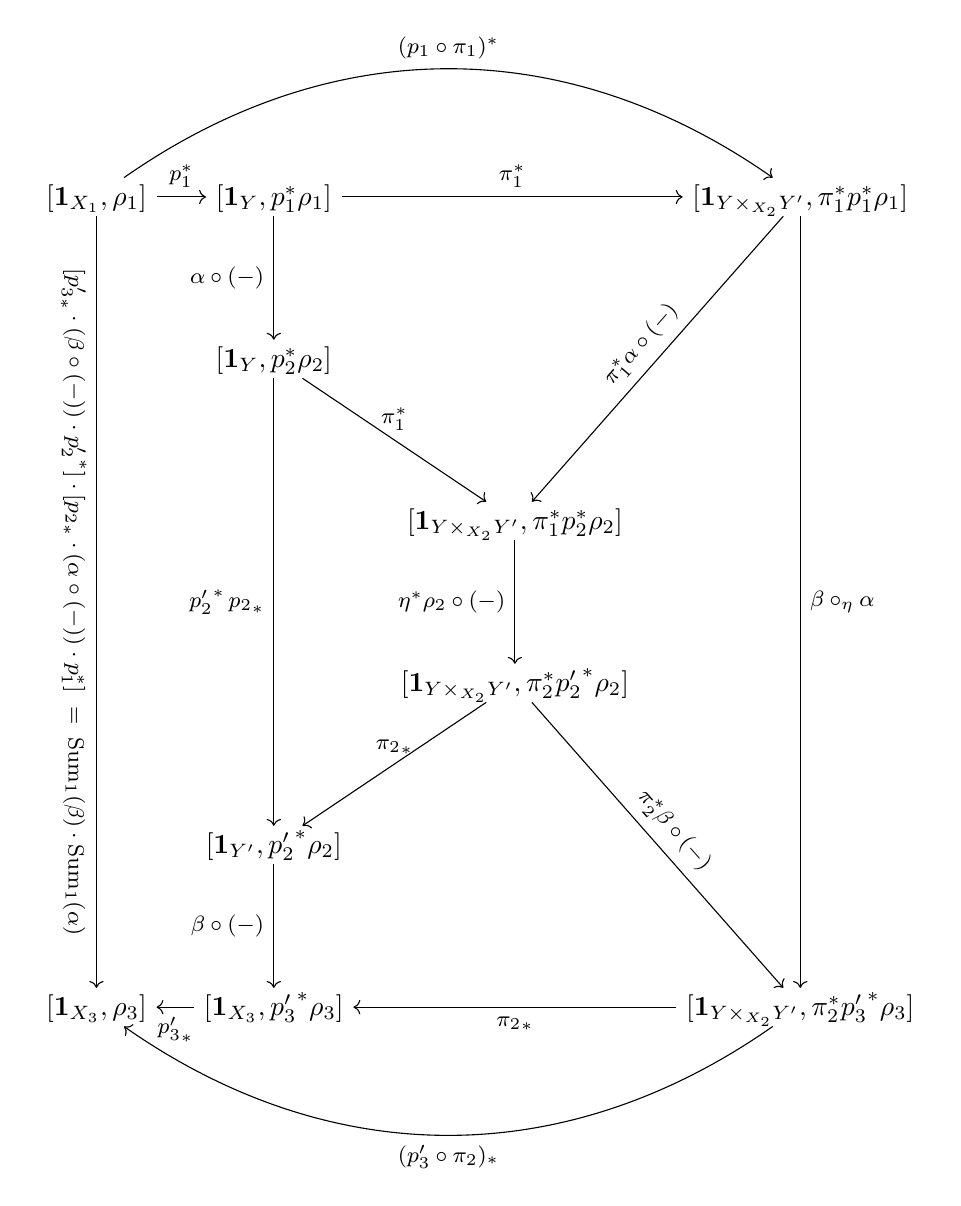
\begin{tikzpicture}[
			     baseline=(current bounding box.base), 
			     %>=stealth,
			     descr/.style={fill=white,inner sep=3.5pt}, 
			     normal line/.style={->}
			     ] 
\matrix (m) [matrix of math nodes, row sep=4.5em, column sep=1.4em, text height=1.5ex, text depth=0.1ex] {%
[\mathbf{1}_{X_1},\rho_1]  &  {}[\mathbf{1}_{Y}, p^*_1\rho_1]   &  {}  &   {}[\mathbf{1}_{Y \times_{X_2} Y'}, \pi_1^* p_1^*\rho_1]
\\
  & {}[\mathbf{1}_{Y}, p_2^*\rho_2] & {} & 
\\
  & {} & {}[\mathbf{1}_{Y \times_{X_2} Y'}, \pi_1^* p_2^* \rho_2] & 
\\
  & {} & {}[\mathbf{1}_{Y \times_{X_2} Y'}, \pi_2^* {p'_2}^* \rho_2] & 
\\
  & {}[\mathbf{1}_{Y'}, {p'_2}^* \rho_2] & {} & 
\\
{}[\mathbf{1}_{X_3},\rho_3]  &  {}[\mathbf{1}_{X_3}, {p'_3}^* \rho_3]   &  {}  &  {}[\mathbf{1}_{Y \times_{X_2} Y'}, \pi_2^* {p'_3}^*\rho_3]
\\
};
\path[font=\footnotesize] (m-1-1) edge[->, out= 35, in= 145] node[sloped, above] {$(p_1\circ \pi_1)^*$} (m-1-4);
\path[font=\footnotesize] (m-1-1) edge[->] node[above] {$p_1^*$} (m-1-2);
\path[font=\footnotesize] (m-1-2) edge[->] node[above] {$\pi_1^*$} (m-1-4);
\path[font=\footnotesize] (m-1-2) edge[->] node[left] {$\alpha\circ(-)$} (m-2-2);
\path[font=\footnotesize] (m-2-2) edge[->] node[above] {$\pi_1^*$} (m-3-3);
\path[font=\footnotesize] (m-2-2) edge[->] node[left] {${p'_2}^* \, {p_2}_*$} (m-5-2);
\path[font=\footnotesize] (m-1-4) edge[->] node[sloped, above] {$\pi_1^*\alpha\circ(-)$} (m-3-3);
\path[font=\footnotesize] (m-1-4) edge[->] node[right] {$\beta \circ_\eta \alpha$} (m-6-4);
\path[font=\footnotesize] (m-3-3) edge[->] node[left] {$\eta^*\rho_2 \circ (-)$} (m-4-3);
\path[font=\footnotesize] (m-4-3) edge[->] node[above] {${\pi_2}_*$} (m-5-2);
\path[font=\footnotesize] (m-4-3) edge[->] node[sloped, above] {$\pi_2^*\beta\circ(-)$} (m-6-4);
\path[font=\footnotesize] (m-5-2) edge[->] node[left] {$\beta\circ(-)$} (m-6-2);
\path[font=\footnotesize] (m-6-4) edge[->] node[below] {${\pi_2}_*$} (m-6-2);
\path[font=\footnotesize] (m-6-2) edge[->] node[below] {${p'_3}_*$} (m-6-1);
\path[font=\footnotesize] (m-1-1) edge[->] node[sloped, below] {$[{p'_3}_* \cdot (\beta\circ(-)) \cdot {p'_2}^*] \cdot [{p_2}_* \cdot (\alpha\circ(-)) \cdot p_1^*] \; = \; \text{Sum}_1(\beta) \cdot \text{Sum}_1 (\alpha)$} (m-6-1);
\path[font=\footnotesize] (m-6-4) edge[->, out= -145, in= -35] node[sloped, below] {$(p'_3\circ \pi_2)_*$} (m-6-1);
\end{tikzpicture}
%%%%%%%%%%%%%%%%%%%%%%% 
$$
The leftmost vertical arrow is $\textrm{Sum}_1(\beta) \circ \textrm{Sum}_1(\alpha)$, hence we are done if we can show that the diagram commutes. 
This is indeed the case: 
the leftmost and rightmost subdiagrams commute by definition, as does the other subdiagram involving $\pi_1^*\alpha\circ(-)$; 
that the top and bottom diagrams commute follows from the definition of pullback and pushforward; 
finally, the subdiagram involving $\pi_2^*\beta\circ(-)$ and ${\pi_2}_*$ commutes by the projection formula of Lemma~\ref{lem:projectionformula}, 
and the middle subdiagram commutes thanks to the Beck-Chevalley condition of Lemma~\ref{lem:BeckChevalley}. 

Finally, if $\rho_2=\rho_3$, $Y=Y'$ and $\beta$ is the identity on $\rho_2$ in $\textrm{Fam}_1(\Vect)$, then $Y \times_{X_2} Y'$ is canonically equivalent to~$Y$, and we see that $\textrm{Sum}_1$ sends units to units. 
\end{proof}





\end{document}